\def\layersep{5em}
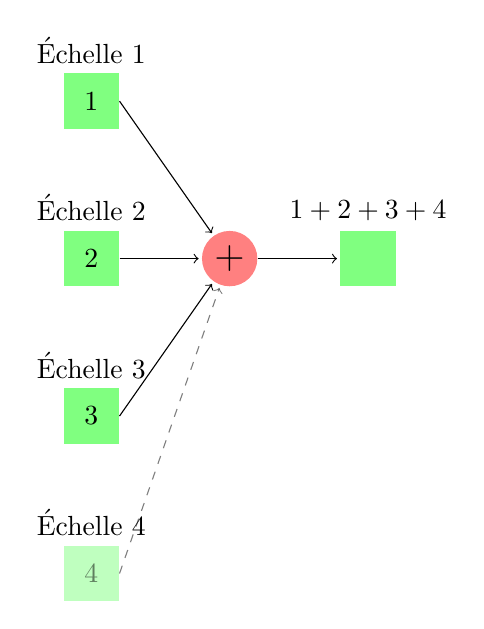
\begin{tikzpicture}[shorten >=1pt,->,draw=black, node distance=\layersep]
\tikzstyle{every pin edge}=[<-,shorten <=1pt]
\tikzstyle{block}=[minimum size=2em];
\tikzstyle{value}=[rectangle, fill=green!50,block];
\tikzstyle{operation}=[block, circle,inner sep=0pt, fill=red!50];
\tikzstyle{nonlinearity}=[rectangle,block, fill=blue!50];
\tikzstyle{annot} = [text width=6em, text centered]

% Draw the input layer nodes
\foreach \name / \y in {1,...,3}
% This is the same as writing \foreach \name / \y in {1/1,2/2,3/3,4/4}
\node[value, label={[]north:{\'{E}chelle \y}}] (I-\name) at (0,-2*\y) {\y};
\node[value, label={[]north:{\'{E}chelle 4}}, opacity=.5] (I-4) at (0,-8) {4};

% Draw the output layer node
\node[operation, right of=I-2] (ope) {{\Large +}};
\node[value, right of=ope, label={[]north:$1+2+3+4$}](cat){};
% Draw the output layer node
%\node[nonlinearity, right of=cat] (lin) {Lin};
%\node[annot, right of=lin, text width=7em,xshift=2em ] (out) {Distribution de probabilit\'{e}s};

% Connect every node in the input layer with every node in the
% hidden layer.
\foreach \source in {1,...,3}
\path (I-\source.east) edge (ope);
\path (I-4.east) edge[dashed, opacity=.5] (ope);
\path (ope) edge (cat);
%\path (cat) edge (lin);
%\path (lin) edge (out);
\end{tikzpicture}